\documentclass[11pt,a4paper]{article}

\usepackage[margin=1in]{geometry}
\usepackage{hyperref}
\usepackage{rotating}
\usepackage[table]{xcolor}
\usepackage[style=authortitle,backend=bibtex,autocite=footnote,bibencoding=ascii]{biblatex}
\usepackage[tocindentauto]{tocstyle}
\usetocstyle{KOMAlike}
\usepackage[english]{babel}
\usepackage{array}
\usepackage{graphicx}
\usepackage{lscape}
\usepackage{tikz-qtree,tikz-qtree-compat}
\usepackage[compact]{titlesec}
\usepackage{fancyhdr}
\usepackage{nomencl}
\usepackage[printonlyused]{acronym}
\usepackage{tablefootnote}
\usepackage{tabularx}
\usepackage{ragged2e}
\usepackage{color}
\usepackage{gensymb}
\usepackage{amsmath}
\usepackage{footnote}
\usepackage{subcaption}
\usepackage{pgfplots}
\usepackage{eurosym}
\usepackage{tikz}
\usepackage{enumitem}
\usepackage{multicol}
\usepackage{multirow}
\usepackage{calc}

%Settings
\setlist[itemize]{noitemsep, topsep=2pt}
\setlength\parindent{0pt}


%Title
\title{Reading 1}
\author{Ali Ul Haq}
\date{February 2016}
 
\begin{document}

\maketitle

An visualisation has been chosen to answer questions according to the following articles: 
\begin{itemize}[noitemsep]
	\item The Functional Art: An introduction to information graphics and visualisation, by Albert Cairo 
	\item Considering Visual Variables as a Basis for Information Visualisation, by S. Carpendale
\end{itemize}


\section*{Questions}
The questions which have to be answered are as following:
\begin{itemize}[noitemsep]
	\item Find a visualisation online and answer the following questions pertaining to that visualisation. Attach the visualisation as a screenshot in your submission.
	\item Consider Bertin’s characterisation of visual variables (position, size, shape, value, color, orientation, and texture). Pick 2 of Bertin’s visual variables, and discuss them in relation to your visualization.
	\item Do you agree that visualisation is a functional art? Explain.
	\item Ask yourself what the designer is trying to convey and think of three to four possible tasks this visualisation should help you with. Does the visualisation achieve any of your tasks? (To view an example, see Albert Cairo, pages 26-­28.)
\end{itemize}

\section{Q1}
The visualisation chosen uses data from the World Banks using the an World development Indicator for internet users (a full size image is shown in appendix 1). It is shared by jkan on visual.ly. The creator of this visualisation is Juuso K\"{a}nk\"{a}nen.

\begin{figure*}[ht]
\centering
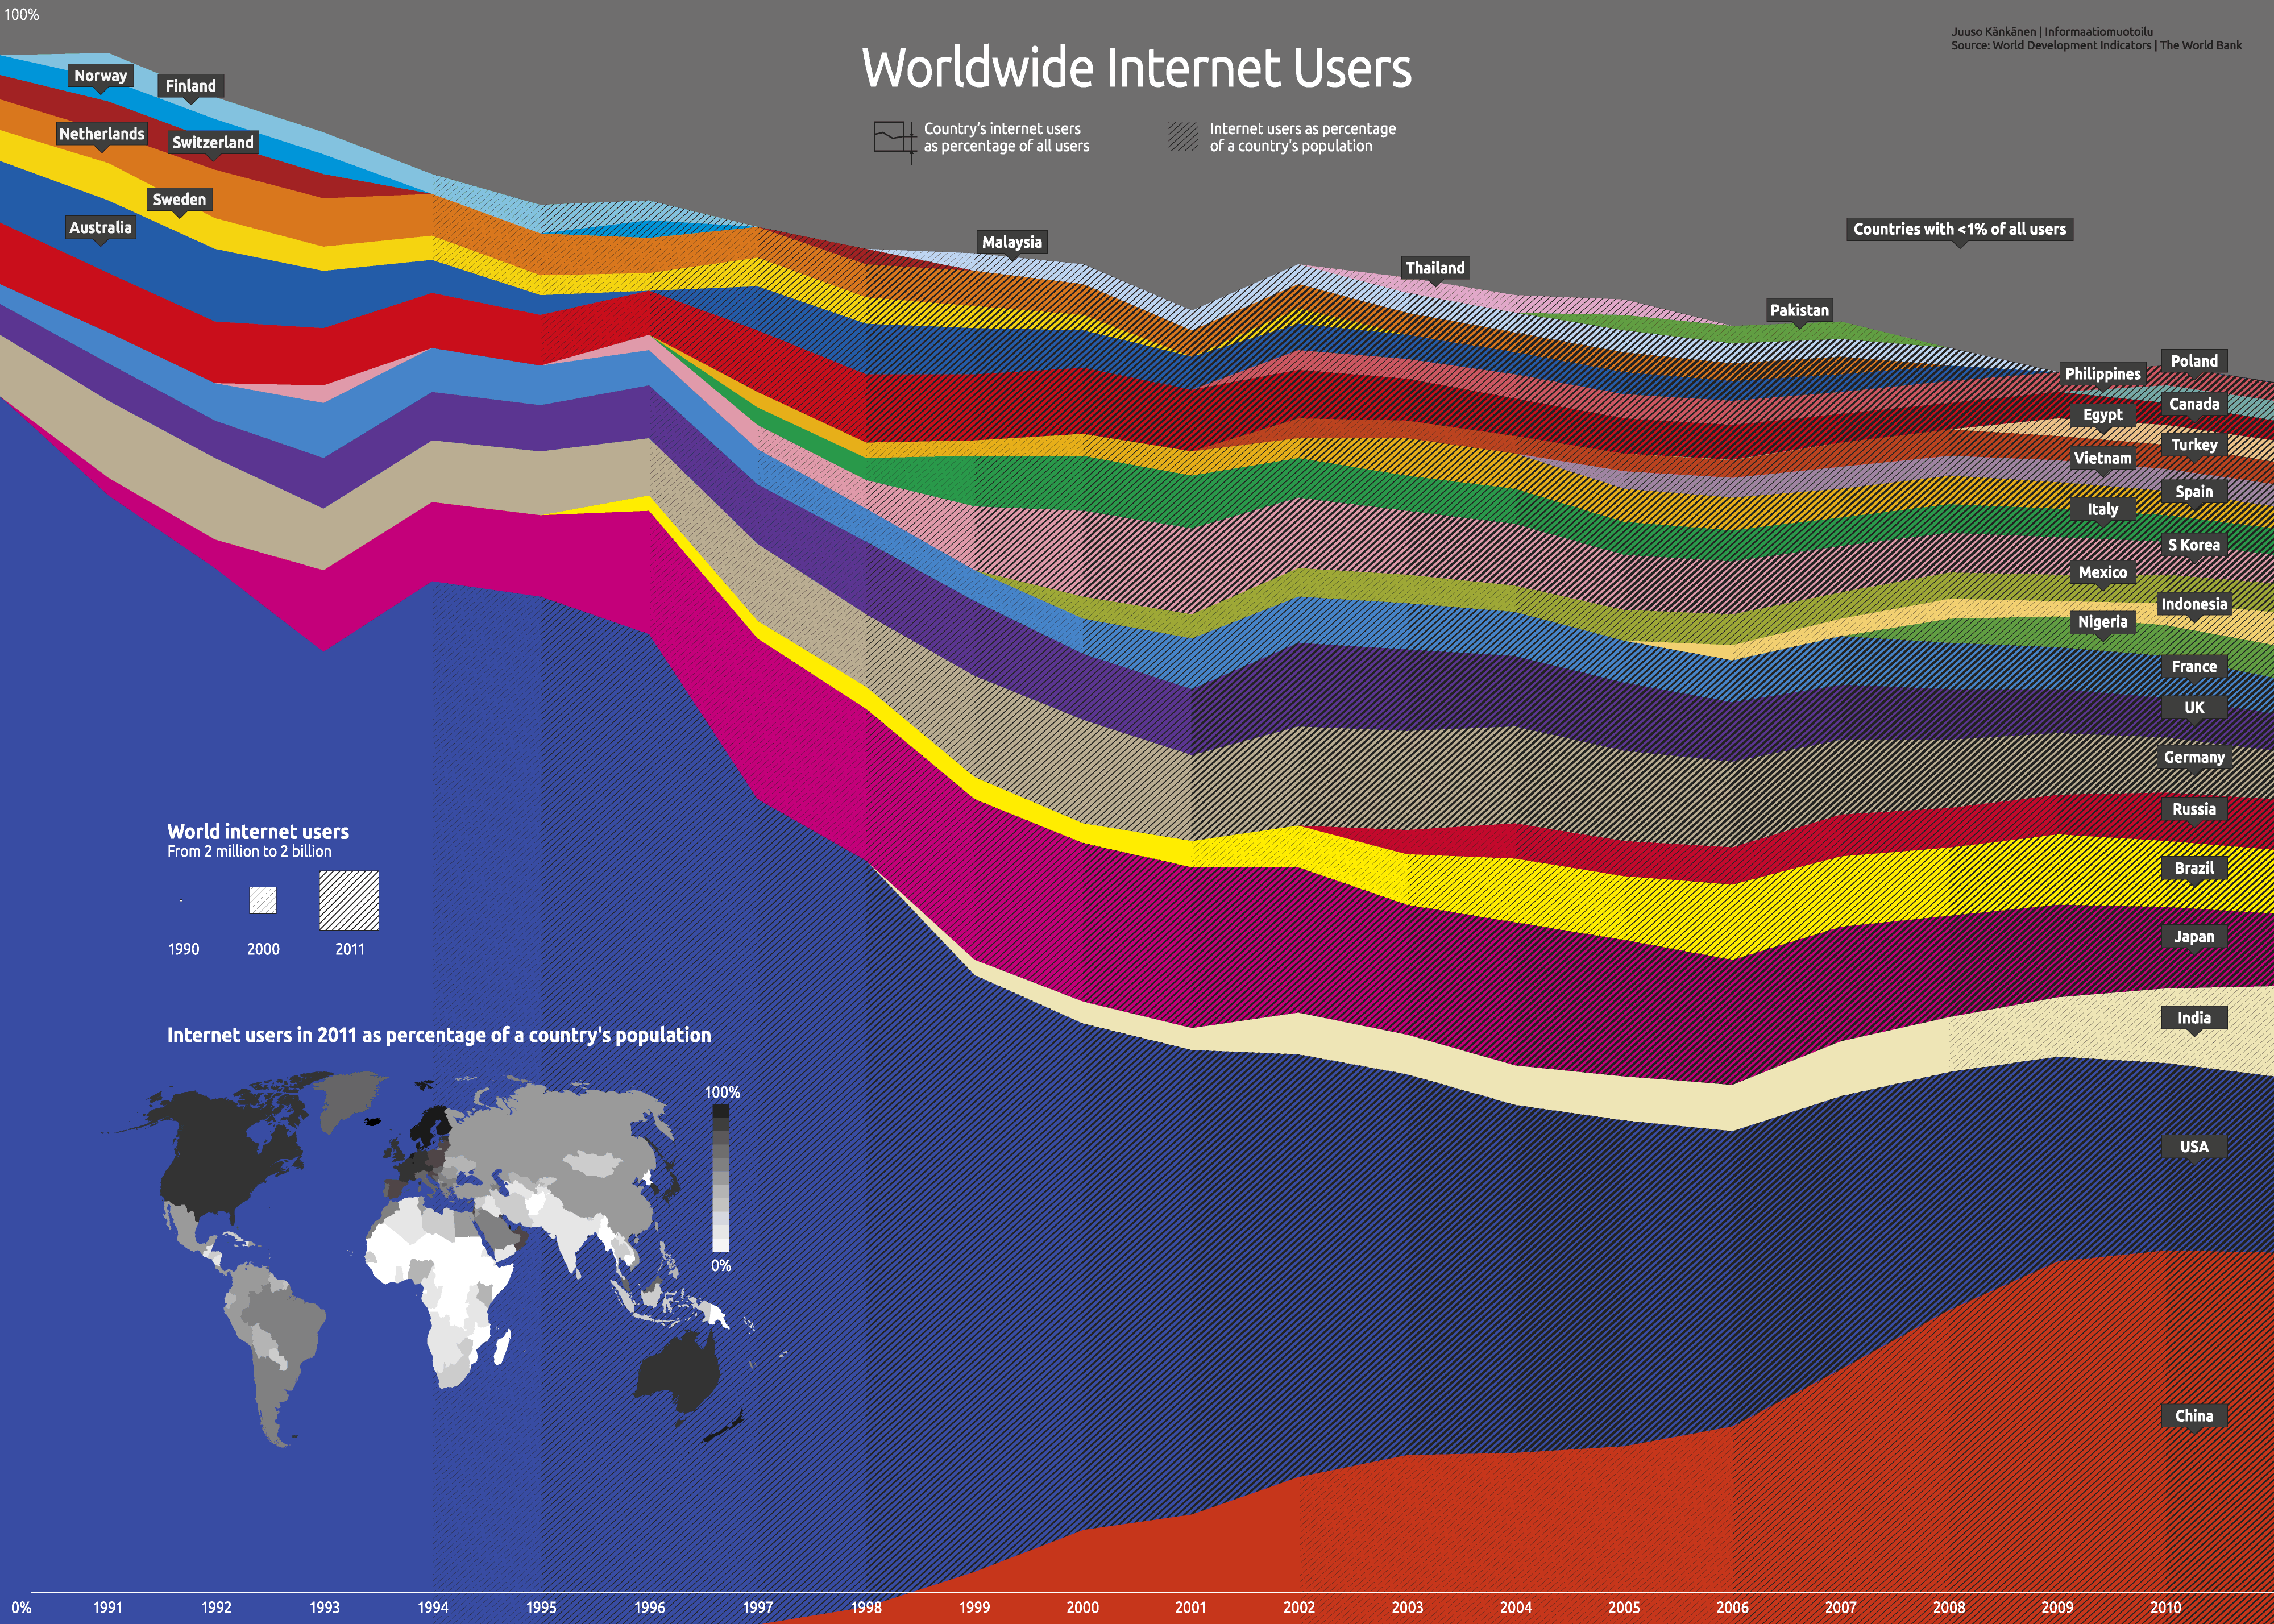
\includegraphics[scale=0.08]{visualisation1}	
\caption*{Worldwide Internet users}
\end{figure*}

\section{Q2}
From Bertins visual variables two have been chosen and will be discussed in relation to the chosen visualisation. The first visual variable is colour (\ref{subsec:colour}) and the second variable is grain (\ref{subsec:grain}). For each variable the existing characteristic will be discussed.\\

\subsection{Colour}\label{subsec:colour}
For this visualisation colour is a primary visual variable due to the fact that each country has its own respective colour to visualise the division of percentage for the countries. 
The following characteristics will be discussed for this visual variable: 

\begin{itemize}[noitemsep]
	\item Selective
	\item Associative
	\item Quantitive
	\item Order
	\item Length
\end{itemize}

\subsubsection{Selective}
There exist a selective characteristic due to the fact that every country has its own colour to represent the percentage shared for each character. This allows it to show a clear separation between each country. The colours are also not similar to the colours used for the world map.
\subsubsection{Associative}
There is no associative characteristic because each country has its own colour and there is no grouping with other countries, for example for each continent. Furthermore colours of the countries are not linked to the world map shown in the corner.
\subsubsection{Quantitive}
Not applicable
\subsubsection{Order}
There is no clear ordering of the colour due to each country having their own colour. Furthermore it also seems like no particular pattern was used to represent the different countries. 
\subsubsection{Length}
The length is primarily used for dark color with some light colours in-between the countries. Furthermore a dark and light black and white is used for the world map.

\subsection{Grain}\label{subsec:grain}
The grain for this visualisation shows the percentage of internet users that exist within the population of the country. It shows the increase of internet users with a thicker line.
The following characteristics will be discussed for this visual variable:

\begin{itemize}[noitemsep]
	\item Selective
	\item Associative
	\item Quantitive
	\item Order
	\item Length
\end{itemize}

\subsubsection{Selective}
There is no different type of grain used for each country. The grain is divided in three types based upon the amount of internet users. 
\subsubsection{Associative}
There is no grouping.
\subsubsection{Quantitive}
Not applicable.
\subsubsection{Order}
Not applicable.
\subsubsection{Length}
Three different grain types are used.

\section{Q3}
I do think that visualisations is a functional art. From what I have understood I've seen that infographics for example use primarly data that is put in by the user itself and therefore the data that is presented can be shown in different forms. Data visualisations are mostly visualisations that is processed from data and therefore automatically generated. Most visualisations can consist as a simple graph or chart depending on the data type. But when the dataset is larger it can be processed to an more arbitrary form but it still serves its purpose to inform the public. This may be done in an artful form, which also has an function.

\section{Q4}
When looking at this graph the artist may want to provide the public about the difference in internet usage world wide. This is emphasised with  world maps shown in the left corner. It provides me with te following information or tasks:

\begin{enumerate}[noitemsep]
	\item It helps me to \textbf{compare} the internet users that exist around the world and the percentage of population that uses the internet.
	\item It helps me to \textbf{organise} the internet usage per country and informs me which countries has the most internet users in the world and how many people use the internet for that respective country.
	\item It does not \textbf{correlate} me with other data, such as GDP or internet speeds within that country, which may be interesting to correlate with.
	\item It does not \textbf{present} me other than the amount of people that use internet within that country.
\end{enumerate}


\begin{sidewaysfigure*}
\section*{Appendix 1}
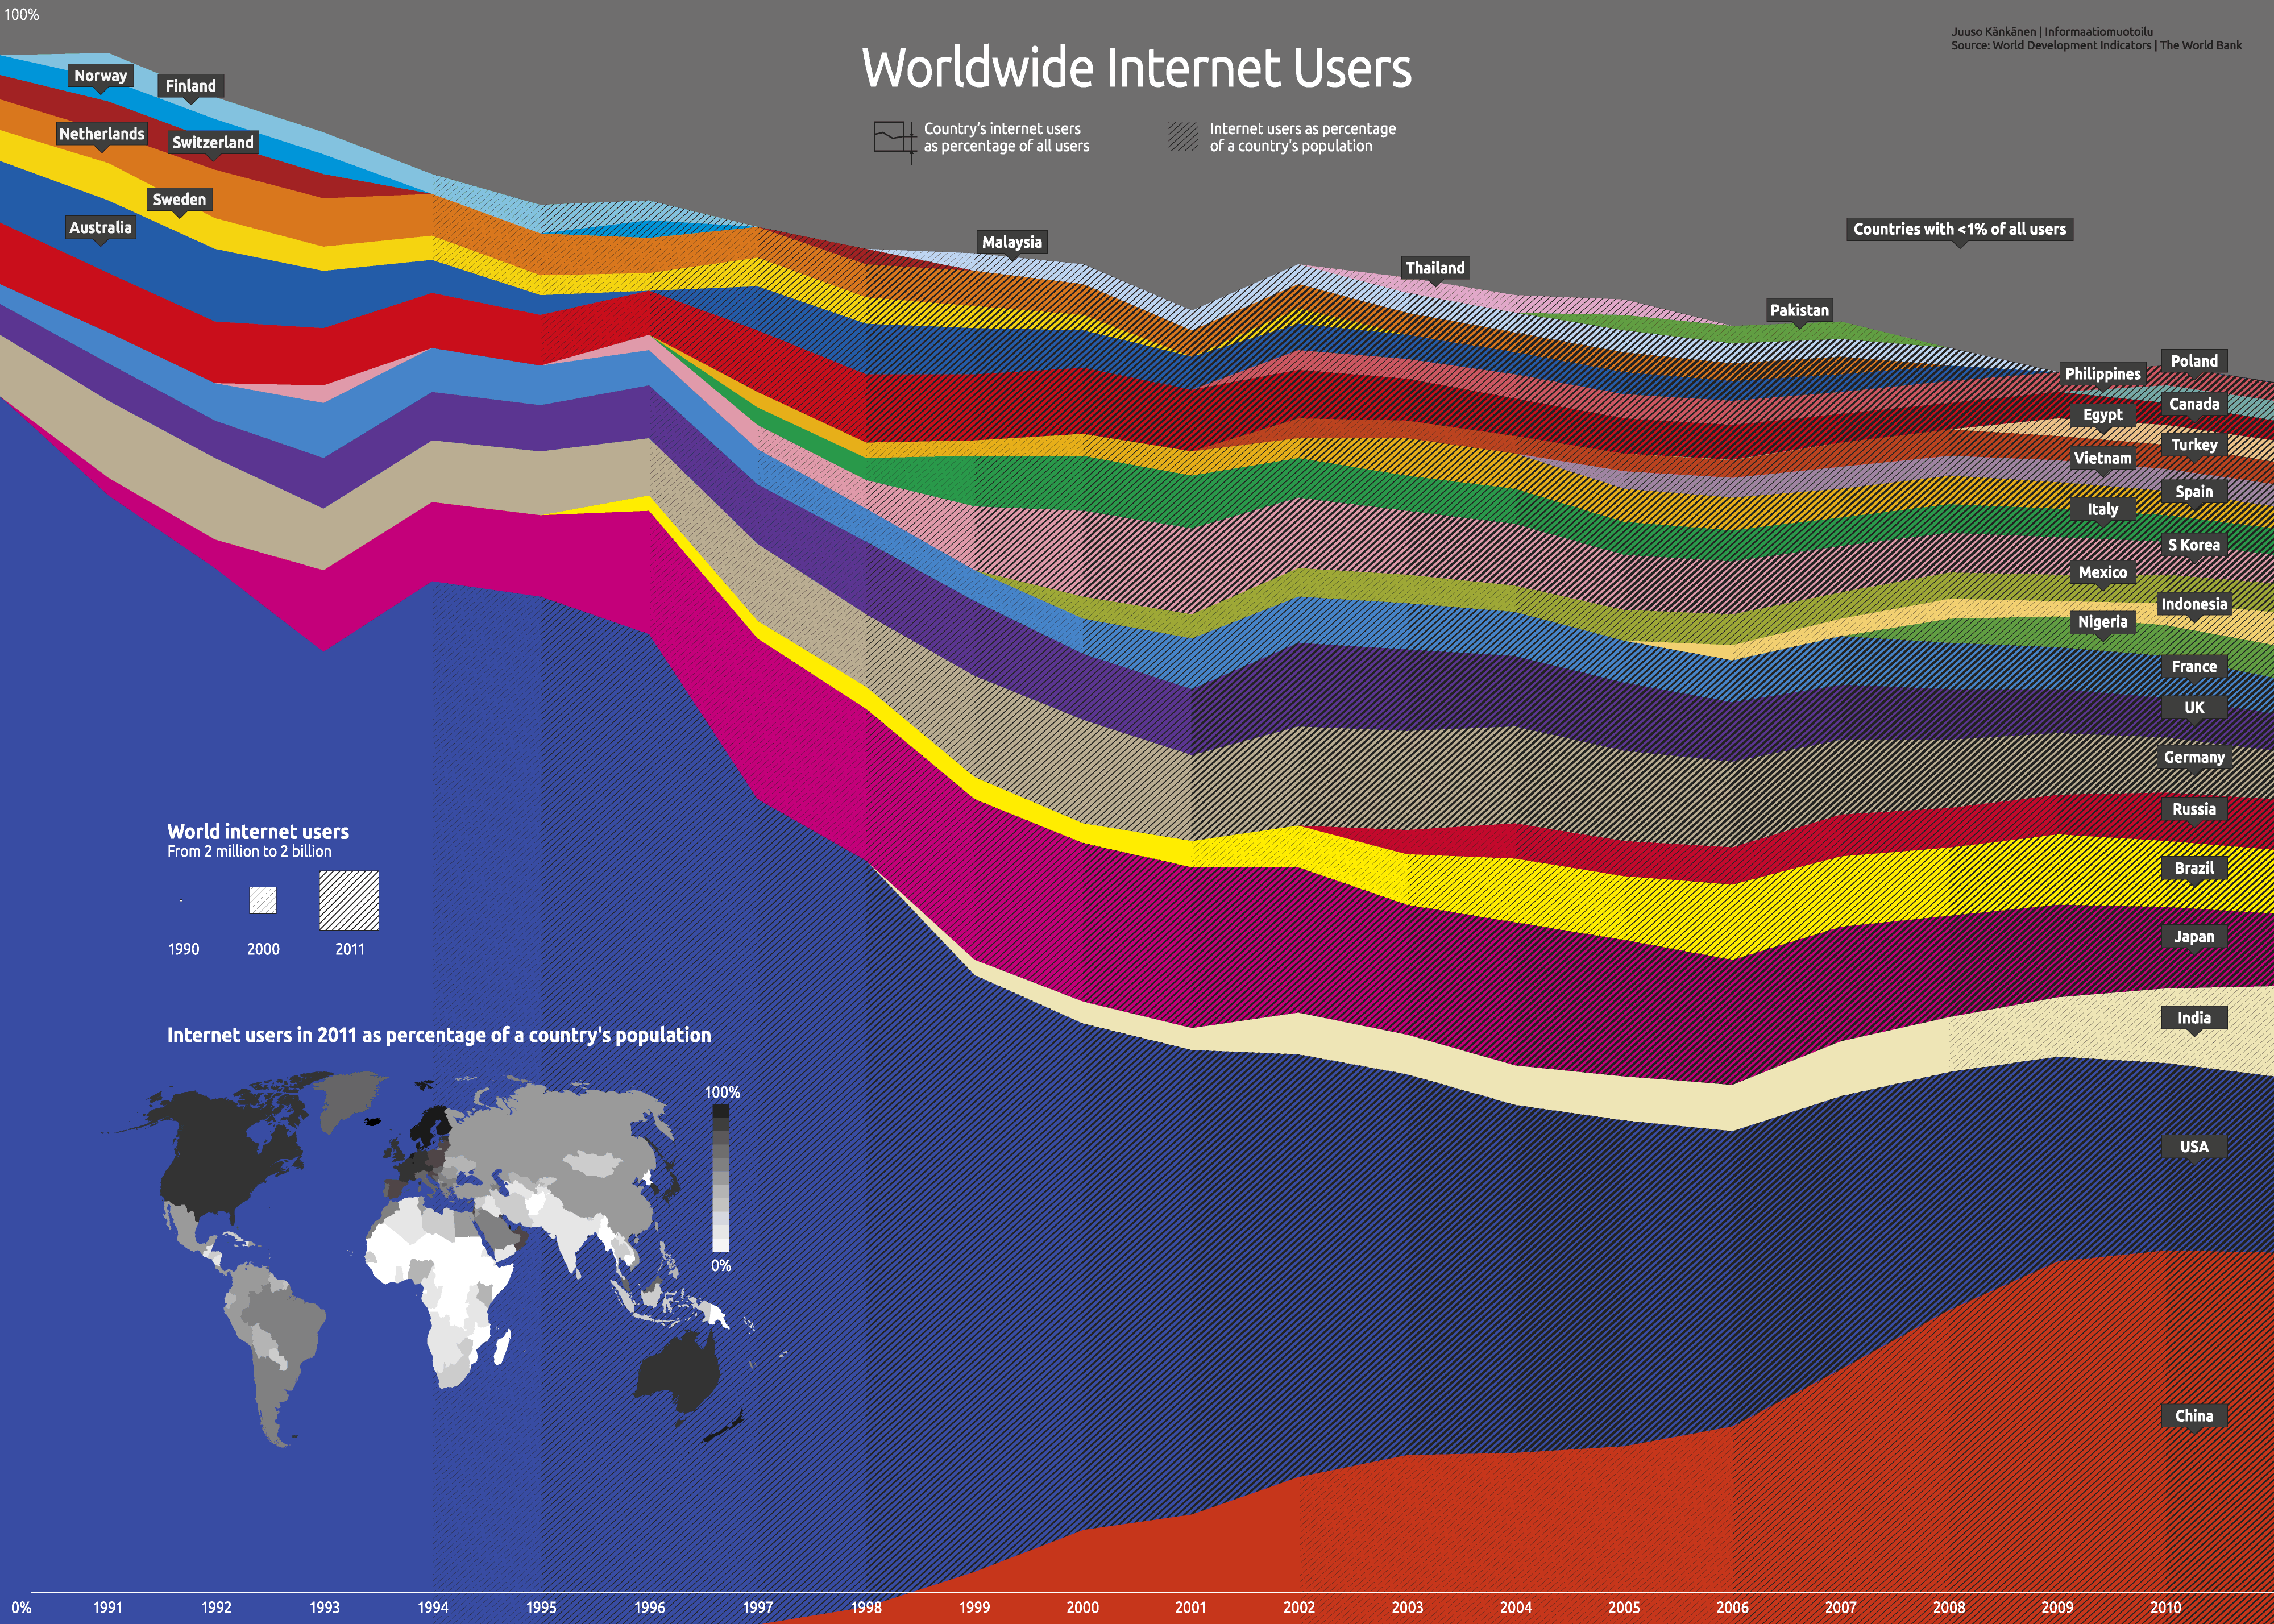
\includegraphics[scale=0.18]{visualisation1}		
\end{sidewaysfigure*}



\end{document}